\documentclass[10pt]{beamer}
\usetheme[progressbar=frametitle]{metropolis}
\includeonlyframes{}
%%%%%%%%%%%%%%%%%%%%%%%%%%%%%%%%%%%%%%%%%%%%%%%%%%%%%%%%%%%%%%%%%%%%%%%%%%%%%%%%
%                           Preambulo                                          %
%%%%%%%%%%%%%%%%%%%%%%%%%%%%%%%%%%%%%%%%%%%%%%%%%%%%%%%%%%%%%%%%%%%%%%%%%%%%%%%%
\usepackage[english]{babel}
\usepackage{xcolor}
\usepackage{color}
\usepackage{colortbl}
\usepackage{amsmath}
\usepackage{amssymb}
\usepackage{graphicx}
\usepackage{latexsym}
\usepackage{ucs}
\usepackage[utf8x]{inputenc}
\usepackage{wrapfig}
\usepackage{siunitx}
\usepackage{times}
\usepackage{tikz}
\usepackage{verbatim}
\usepackage{multimedia}
\usepackage{hyperref}
\usepackage{thumbpdf}
\usepackage{wasysym}
\usepackage{pgf, pgfarrows, pgfnodes, pgfautomata, pgfheaps, pgfshade}
\usepackage{url}
\usepackage{empheq}
\usepackage{fancybox}
\usepackage{esint}
\usepackage{lipsum}
\usepackage{listings}
\usepackage{mathptmx}
\usepackage{helvet}
\usepackage{tikz}%
\usepackage{circuitikz}
\usepackage{csvsimple}
\usepackage{pgfplots}
\usepackage{multimedia}
\usepackage{media9}
\usepackage{proba}
\usepackage[absolute,overlay]{textpos}
\usepackage{bibunits}
\usepackage{tcolorbox}
\usepackage{booktabs}
% \usepackage[
% texcoord,
% grid, gridunit=mm, gridcolor=red!60,
% subgridcolor=green!60]%
% {eso-pic}
\usepackage[makeroom]{cancel}
\usepackage{epstopdf}
\usepackage{algorithm}
\usepackage{algorithmic}
\newcommand{\s}{\subseteq}
\newcommand{\e}{\varepsilon}
%
\epstopdfsetup{outdir=./}
\newcommand{\themename}{\textbf{\textsc{metropolis}}\xspace}
\title{%
    EXISTENCE,
    CHARACTERIZATION AND SIMULATION OF OPTIMAL
    POLICIES IN A FAMILY OF EPIDEMIC MODELS
    \\
    \small{
        (%
        \textsc{%
            S. D\'iaz-Infante, %
            F. Pe\~n\'u\~nuri, %
            D. Gonz\'alez-S\'anchez,
        } In press.)
        \\%
        Part of the thesis:
        Optimal Control Applied in Epidemic Models.
        \\
        N. Palafox Lacarra.
        }{}
}
\subtitle{XXIX SNIDM}
\date{\today}
\author{Sa\'ul D\'iaz Infante Velasco}
\institute{CONACYT-Universidad de Sonora}
\titlegraphic{
    \vspace{-2em}
    \hfill
    
\includegraphics[scale=.05]{logoSemanaxxixUnison.png}
}
\metroset{block=fill}
%%%%%%%%%%%%%%%%%%%%%%%%%%%%%%%%%%%%%%%%%%%%%%%%%%%%%%%%%%%%%%%%%%%%%%%%%%%%%%%%
\def\Q#1#2{\frac{\partial #1}{\partial #2}}
\usetikzlibrary{arrows,shapes}
%%%%%%%%%%%%%%%%%%%%%%%%%%%%%%%%%%%%%%%%%%%%%%%%%%%%%%%%%%%%%%%%%%%%%%%%%%%%%%%%
%------------------------------------Theorems 
\newtheorem{remark}{Remark}
\newtheorem{proposition}{Proposition}
%-----------------------------ExtrasDeTercerPresentacion
%--------------------------------Fancyboxes-------------------------------------
\definecolor{myblue}{rgb}{.8, .8, 1}
\definecolor{shadecolor}{cmyk}{0,0,0.41,0}
\newcommand*\mybluebox[1]{%
	\colorbox{myblue}{\hspace{1em}#1\hspace{1em}}
}
\newcommand*\myyellowbox[1]{%
	\colorbox{darkyellow}{\hspace{1em}#1\hspace{1em}}
}
%--------------------------------------------------------------------------
\definecolor{shadecolor}{cmyk}{0,0,0.41,0}
\definecolor{light-blue}{cmyk}{0.25,0,0,0}
\newsavebox{\mysaveboxM} % M for math
\newsavebox{\mysaveboxT} % T for text
\newcommand*\Garybox[2][Example]{%
	\sbox{\mysaveboxM}{#2}%
		\sbox{\mysaveboxT}{\fcolorbox{black}{light-blue}{#1}}%
			\sbox{\mysaveboxM}{%
	\parbox[b][\ht\mysaveboxM+.5\ht\mysaveboxT+.5\dp\mysaveboxT][b]{%
		\wd\mysaveboxM}{#2}%
	}%
	\sbox{\mysaveboxM}{%
		\fcolorbox{black}{shadecolor}{%
		\makebox[\linewidth-10em]{\usebox{\mysaveboxM}}%
		}%
	}%
	\usebox{\mysaveboxM}%
	\makebox[0pt][r]{%
		\makebox[\wd\mysaveboxM][c]{%
			\raisebox{\ht\mysaveboxM-0.5\ht\mysaveboxT
			+0.5\dp\mysaveboxT-0.5\fboxrule}{\usebox{\mysaveboxT}}%
		}%
	}%
}
\newcommand\Fontvi{\fontsize{7}{7.2}\selectfont}
%%%%%%%%%%%%%%%%%%%%%%%%%%%%%%%%%%%%%%%%%%%%
\definecolor{kugreen}{RGB}{50,93,61}
\definecolor{kugreenlys}{RGB}{132,158,139}
\definecolor{kugreenlyslys}{RGB}{173,190,177}
\definecolor{kugreenlyslyslys}{RGB}{214,223,216}
\definecolor{greenArea}{RGB}{124,252,124}
\definecolor{hellmagenta}{rgb}{1,0.75,0.9}
\definecolor{hellcyan}{rgb}{0.75,1,0.9}
\definecolor{hellgelb}{rgb}{1,1,0.8}
\definecolor{colKeys}{rgb}{0,0,1}
\definecolor{colIdentifier}{rgb}{0,0,0}
\definecolor{colComments}{rgb}{1,0,0}
\definecolor{colString}{rgb}{0,0.5,0}
\definecolor{darkyellow}{rgb}{1,0.9,0}
\setbeamercovered{transparent}
\lstset{%
    language=[AlLaTeX]TEX,%
    float=hbp,%
    basicstyle=\ttfamily\small, %\usepackage{cir}
    identifierstyle=\color{colIdentifier}, %
    keywordstyle=\color{colKeys}, %
    stringstyle=\color{colString}, %
    commentstyle=\color{colComments}, %
    columns=flexible, %
    tabsize=3, %
    frame=single, %
    extendedchars=true, %
    showspaces=false, %
    showstringspaces=false, %
    numbers=left, %
    numberstyle=\tiny, %
    breaklines=true, %
    backgroundcolor=\color{hellgelb}, %
    breakautoindent=true, %
    captionpos=b,%
    xleftmargin=18pt,%
    xrightmargin=\fboxsep%
}
\pgfplotsset{
    left segments/.code={\pgfmathsetmacro\leftsegments{#1}},
    left segments=3,
    left/.style args={#1:#2}{
        ybar interval,
        domain=#1:#2,
        samples=\leftsegments+1,
        x filter/.code=\pgfmathparse{\pgfmathresult}
       }
}
\DeclareMathOperator{\sign}{sgn}
\newcommand{\innerprod}[2]{\left\langle#1, #2\right\rangle}
\newcommand\bound{10} % bound number of points on each side of N
\newcommand\labelnum[3][]{
	\begin{scope}[font=\footnotesize,x=.3cm,#1]
	  \foreach \mypt in {0,#2,...,\bound}{
	    \draw(\mypt,0)circle[radius=2pt];
	    \draw(-\mypt,0)circle[radius=2pt];
	  }
	  \draw(-\bound-5,0)--(\bound+5,0) node[pos=0, left]{$t$};
	  \node(start)[at={(-\bound-4,0)},label=below:{$t_0=0$}]{$[$};
	  \node(end)[at={(\bound+4,0)},label=below:{$T=Nh$}]{$]$};
	  \node[%
		  at={($(start)!.319!(end)$)},
		  label=below:{
			   $\underbrace{}_{h}$
			}%
			]{\vphantom{$[$}};
	  \node[at={($(start)!.57!(end)$)},label=below:{$t_{n+1}$}]{\vphantom{$[$}};
	  \filldraw(0,0)circle[radius=2pt];
	  \node[at={(-\bound-2,0)},above]{$\cdots$};
	  \node[at={(\bound+2,0)},above]{$\cdots$};
	  \node[at={(0,0)},above=5pt]{#3};
	\end{scope}
}
\tcbuselibrary{skins,breakable}

\author[Sa\'ul D\'iaz Infante Velasco]{
        Sa\'ul D\'iaz Infante Velasco
    }
    \date[\ccbyncsa]{March 7, 2019 }
    \hypersetup{%
        pdfauthor={Saul Diaz-Infante},
        pdfkeywords={latex, features, publicity, preview}
}
\defaultbibliography{references}
\defaultbibliographystyle{plainnat}
\begin{document}
    \begin{frame}[plain]
        \maketitle
    \end{frame}
    \section{Introduction}
        \begin{frame}{}
    \begin{textblock*}{55mm}(5mm, 5mm)
        \begin{beamerboxesrounded}{Speckled monster and control}
                By the end of the Middle Ages, smallpox cut down the
            population in centers of Europe and Asia.

                This  ``monster'' represents the first documented
            disease against which a specific control intervention was
            available: the inoculation.
        \end{beamerboxesrounded}
    \end{textblock*}
%
    \begin{textblock*}{115mm}(5mm, 68mm)
        \begin{beamerboxesrounded}{}
            Then Bernoulli naturally sets a question like this: What
            happens if everybody were inoculated? Here, we address the
            question: \textbf{How to  inoculate in an optimal way?}
        \end{beamerboxesrounded}
    \end{textblock*}
%
    \begin{textblock*}{60mm}(70mm, 5mm)
        \begin{bibunit}[apalike]
            \nocite{bradley1971smallpox, Foppa2017}
            \putbib
        \end{bibunit}
    \end{textblock*}
\end{frame}
%
{%
\setbeamertemplate{background canvas}{%
\hskip-2em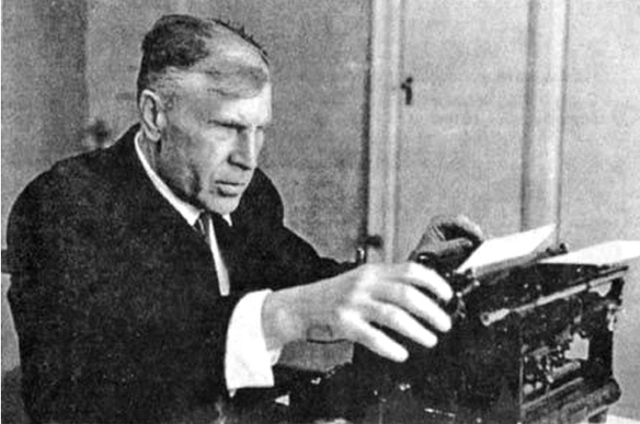
\includegraphics[height=\paperheight]{LevPontriaguin}}
\setbeamercolor{itemize item}{fg=structure.fg!45}
\begin{frame}[plain,t]
    \vfill
    \hfill
    \begin{minipage}{.60\textwidth}
        \usebeamercolor[bg]{normal text}
        \hspace{1em}
        \textbf{\large Lev Semenovich Pontryagin \\
            \hspace*{0.47cm} (1908-1988)}
        \begin{itemize}
        \usebeamercolor[bg]{normal text}
            \item
                Soviet mathematician. He was born in Moscow and lost his
                eyesight due to a primus stove explosion when he was 14.
            \item
                He was able to become one of the greatest
                mathematicians of the 20th century, partially with the help of
                his mother Tatyana Andreevna who read mathematical books and
                papers (notably those of Heinz Hopf, J. H. C. Whitehead, and
                Hassler Whitney) to him.
            \item
                He made major discoveries in a number
                of fields of mathematics, including algebraic topology and
                differential topology.
        \end{itemize}
    \end{minipage}
    \bigskip
\end{frame}
\usebeamercolor[bg]{normal text}
}
%
{%
\setbeamertemplate{background canvas}{%
\hskip-2em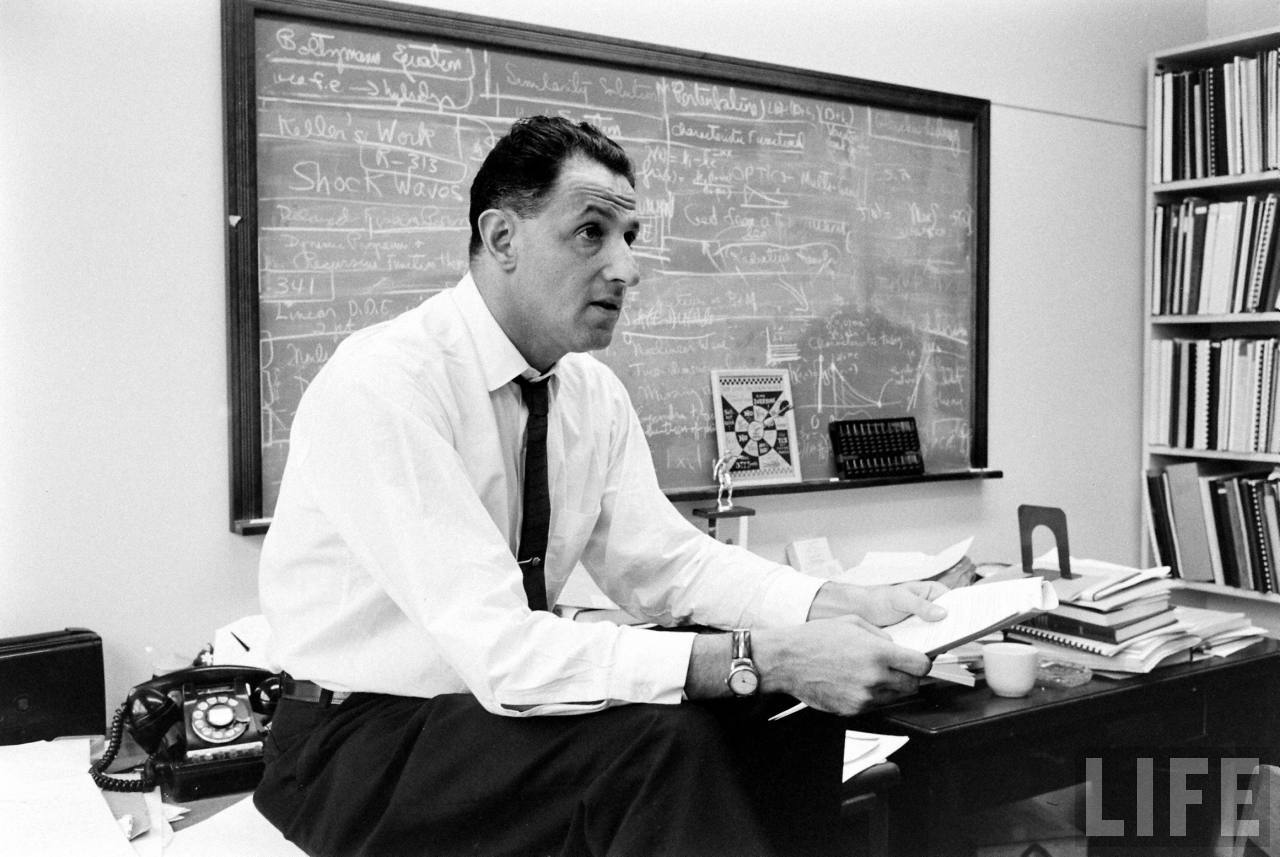
\includegraphics[height=\paperheight]{RichardBellman}}
\setbeamercolor{itemize item}{fg=structure.fg!45}
\begin{frame}

\end{frame}
}

{%
\setbeamertemplate{background canvas}{%
\hskip-2em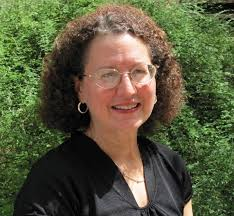
\includegraphics[width=1.2\paperwidth]{SuzanneLenhart}}
\begin{frame}{}
    \only<2->{
    \begin{textblock*}{55mm}(2mm, 5mm)
        \begin{beamerboxesrounded}{Optimal control theory is a way.}
                In the fifties, \textbf{Pontryagin} and
            \textbf{Bellman} propose generalizations of the calculus
            of variations of broader applicability:
            \begin{itemize}
                \item
                    the Maximum Principle
                \item
                    and the method of Dynamic Programming,
            \end{itemize}
            respectively.
        \end{beamerboxesrounded}
    \end{textblock*}
    }
%
    \only<3->{
    \begin{textblock*}{120mm}(5mm, 70mm)
        \begin{beamerboxesrounded}{}
            \begin{bibunit}[apalike]
                \nocite{lenhart2007optimal}
                \putbib
            \end{bibunit}
        \end{beamerboxesrounded}
    \end{textblock*}
    }
\end{frame}
}

        \begin{frame}
            \frametitle{Contents}
            \tableofcontents
        \end{frame}
    \section{Control policies in epidemics}
        {
\begin{frame}{Control policies}
    \begin{textblock*}{55mm}(2mm, 10mm)
        \begin{beamerboxesrounded}{Optimal control theory is a way.}
            \begin{itemize}
                \item \only<2->{
                    We require a \textbf{model} to describe the spreading of an 
                    uncontrolled disease, and whose transitions generate a 
                    \textbf{cost or reward}.
                    }
                \item \only<3->{
                    Continuous \textbf{control action} that modify changes 
                    between states.
                    }
                \item \only<4->{
                    A \textbf{functional} which describes \textbf{cost-reward}.
                    }
            \end{itemize}
        \end{beamerboxesrounded}
    \end{textblock*}
%
    \begin{textblock*}{65mm}(62mm, 10mm)
        \begin{beamerboxesrounded}{Control Policy}
            \begin{itemize}
                \item \only<5->{
                    A rule that prescribes which control
                    operation to use at each time, is a \textbf{control policy}.
                }
                \item \only<6->{
                    \textbf{closed-loop} or \textbf{feedback} control.
                }
                \item \only<7->{
                    \textbf{open-loop} policy.
                }
            \end{itemize}
            %
            \only<8>{
                We consider control policies that affect the bounded rates at which 
                population moves from one class (e.g., infected) to another (e.g., 
                recovered).
            }
        \end{beamerboxesrounded}
    \end{textblock*}
    %
    %
    \begin{textblock*}{90mm}(25mm, 65mm)
        \begin{bibunit}[apalike]
            \nocite{Wickwire1977}
            \putbib
        \end{bibunit}
    \end{textblock*}
\end{frame}
}
        \begin{frame}{SARS: isolation and quarantine}
    \only<1-4>{
    \begin{textblock*}{55mm}(2mm, 12mm)
            If an disease lacks of a rapid diagnostic test, therapy or 
        vaccine, then isolation and quarantine .
%
            Gumel et. al %\cite{Gumel2004}
            model this strategies for (SARS).
    \end{textblock*}
    
    \begin{textblock*}{120mm}(2mm, 62mm)
        \only<1>{
        \begin{bibunit}[apalike]
            \nocite{Gumel2004}
            \putbib
        \end{bibunit}
        }
        \only<2>{
        \begin{bibunit}[apalike]
            \nocite{Yan2008}
            \putbib
        \end{bibunit}
        }
    \end{textblock*}
    }
%        
    \only<2-4>{
    \begin{textblock*}{55mm}(65mm, 12mm)
            Based in the work of Gumel et. al., Yan and Zou report 
            %\cite{Yan2008} 
            a control epidemic model for SARS. They use 
            quarantine and isolation as mitigation controls. 
     \end{textblock*}
    }
%
%
    \only<4-6>{
    \begin{textblock*}{65mm}(17mm, 35mm)
     \begin{equation*}\label{eqn:sars_model}
        \begin{aligned}
            \dfrac{dS}{dt} &=
                \Lambda 
                -\dfrac{
                    S
                    \left(
                        \beta I 
                        + \mathcal{E}_E  \beta E
                        + \mathcal{E}_Q  \beta Q
                        + \mathcal{E}_J  \beta J
                    \right)
                }{N}
                - \mu S,
            \\
            \dfrac{dE}{dt} &=
                p +
                \dfrac{
                    \beta S
                    \left(
                        \beta I 
                            + \mathcal{E}_E \beta E
                            + \mathcal{E}_Q \beta Q
                            + \mathcal{E}_J \beta J
                    \right)
                }
                {N}
                -(
                \only<5->{
                    \textcolor{cyan}{u_1(t)+}
                }
                      k_1 + \mu
                      \only<4>{+\gamma_1}
                )E,
            \\
            \dfrac{dQ}{dt} &=
                \only<5->{
                    \textcolor{cyan}{u_1(t)}
                }
                 \only<4>{\gamma_1}
                 E - (k_2 + \mu) Q,
            \\
            \dfrac{dI}{dt} &=
                k_1 E 
                -(
                \only<5->{
                    \textcolor{cyan}{u_2(t)}
                }
                \only<4>{\gamma_2}
                + d_1  + \sigma_1 
                + \mu) I,
            \\
            \dfrac{dJ}{dt} &=
                \only<5->{
                    \textcolor{cyan}{u_2(t)}
                }
                \only<4>{\gamma_2}  
                  I 
                + k_2 Q
                - (d_2 + \sigma_2 + \mu) J,
            \\
            \dfrac{dR}{dt} &=
                \sigma_1 I
                +\sigma_2 J
                - \mu R.
        \end{aligned}
     \end{equation*}
    \end{textblock*}
    }
    \only<5-6>{
        \begin{textblock*}{55mm}(15mm, 12mm)
            \begin{equation*}\label{eqn:sars_cost}
              \min_{u \in U}\int_{0}^{t_f}
                  \left[
                    B_1 E(t)
                    + B_2 Q(t)
                    + B_3 I(t)
                    + B_4 J(t)
                    + \frac{C_1}{2} u_1^2 (t)
                    + \frac{C_2}{2} u_2^2 (t)
                  \right]
                  dt.
            \end{equation*}
        \end{textblock*}
    }
    
\end{frame}
    \section{Existence and characterization of optimal policies}
        \begin{frame}{Existence and characterization of optimal policies}
    \only<1>{
    \begin{textblock*}{100mm}(15mm, 12mm)
        The non controlled epidemic model described above is of the
        form 
        \begin{eqnarray*}
            \dot{X} & = & AX +  
            \begin{bmatrix}
                X^\top B^{(1)}\\
                \vdots \\
                X^\top B^{(n)}
            \end{bmatrix}X + k  \\
            & = & \left(A + [X^\top \cdots X ^ \top]
            \begin{bmatrix}
                    B^{(1)}\\
                    \vdots \\
                    B^{(n)}
            \end{bmatrix} \right) X + k
        \end{eqnarray*}
        where the matrix $A$ represents the linear part of the system, each 
        matrix $B^{(j)}$, $j=1,\ldots,n$, 
        gives the {\it interaction} part as a quadratic 
        form, and $k$ is a constant vector.
        
         Thus the $j$-th row of the above system takes the form 
            \[ \dot{X}_j = r_j(A)X + X^\top B^{(j)}X + k_j.\]
    \end{textblock*}
    }
\end{frame}
%
%
%
\begin{frame}{A family of control systems}
    Let $\mathbf{X} \subset \mathbb{R} ^ n$ and 
    $\mathbf{U} \subset \R^m$ be nonempty 
    and compact sets. The sets $\mathbf{X}$ and $\mathbf{U}$ are 
    respectively called the {\it state space} and the {\it control space}. The 
    vectors in $X$ have non-negative entries, in particular we assume that 
    $0\in X$. The control set $\mathbf{U}$ is convex. We consider the following 
    control system, for $j=1,\ldots,n$, 
    \begin{equation*}
        \dot{X}_j  =  [r_j(A) + u^\top C^{(j)}]X +
        X^\top    \begin{bmatrix}
        r_1(B^{(j)}) + u^\top D^{(j1)}\\
        \vdots \\
        r_n(B^{(j)}) + u^\top D^{(jn)}
      \end{bmatrix}  X + k_j
    \end{equation*}
    where $A\in\R^{n\times n}$,
    $B^{(j)}\in\R^{n\times n}$, 
    $C^{(j)}\in\R^{m\times n}$,
    and $ D^{(jl)}\in\R^{m\times n}$ for $l=1,\ldots,n$.
\end{frame}
%
%
%
%
\begin{frame}{}
    \begin{equation*}
        \dot{X}_j  =  [r_j(A) + u^\top C^{(j)}]X +
        X^\top    \begin{bmatrix}
        r_1(B^{(j)}) + u^\top D^{(j1)}\\
        \vdots \\
        r_n(B^{(j)}) + u^\top D^{(jn)}
      \end{bmatrix}  X + k_j, \quad j=1,\dots, n.
    \end{equation*}
%
    \begin{theorem}
        For each measurable function 
        $u:[0,T]\to \mathbf{U}$ and each initial condition $x_0\in X$,
        there exists a unique absolutely continuous function 
        $X_u:[0,T]\to \R^n$ that satisfies the the 
        system  almost everywhere. 
    \end{theorem}
\end{frame}
%
%
%
\begin{frame}{Existence of optimal policies.}
    Consider the  {\it cost functional} of an admissible control $u$, given the 
    initial state $x_0$, 
    \begin{equation}\label{CostFunctional} 
        V(u,x_0) := \int_0 ^ T g(X(t), u(t)) \ ,dt,
    \end{equation}
    %
    where $g: \mathbf{X} \times \mathbf{U} \to \R$ is continuous. 
    The {\it optimal control problem} (OCP) consists of finding an admissible 
    control $u^\ast$ such that
    \[ V(u^\ast,x_0)=\inf\{ V(u,x_0)\mid u\in \mathbb{U}_B \}.\]
    If there exists such a control $u^\ast$, then it is called an 
    {\it optimal policy} or {\it optimal control}. 
    The pair $(u^\ast,X^\ast)$, where $X^\ast$ is given by 
    the above Theorem, is an {\it optimal pair}.
\end{frame}

        \begin{frame}{Sufficient conditions for optimality}
    Consider the Hamiltonian 
    $
        \mathcal{H}:\mathbf{X}\times\mathbf{U}\times\R^n\to \R
    $, defined as 
    \[
        \mathcal{H}(x, u, \lambda):=
             g(x,u) + \lambda ^ \top f(x,u),
    \]
        and
        \[ 
            \mathcal{H}^\ast(x,\lambda)  
            := \inf_{u\in\mathbf{U}}\mathcal{H}(x,u,\lambda),
        \]
        where $g$ determines the cost functional 
        and $f$ is given by the right-hand side of the control system.

        The function $\lambda:[0,T]\to \R^n$ and the admissible pair 
        $(u,X)$ satisfy the necessary conditions of the 
        {\it Maximum Principle} (MP) if they solves
        {\it adjoint equation}
        \begin{equation*}
             \dot{\lambda}(t) = -\mathcal{H}_x(X(t),u(t),\lambda(t))^\top, 
             \quad \lambda(T)=0,
        \end{equation*}
        and satisfy the {\it optimality condition}
        \begin{equation*}\label{OptCond}
            \mathcal{H}^\ast(X(t),\lambda(t)) =
            \mathcal{H}(X(t),u(t),\lambda(t)).
       \end{equation*}
\end{frame}

\begin{frame}{}
    \begin{definition}\label{PiecewiseCont}
        \rm The function $w$ from $[0,T]$ to some Euclidean space is {\it 
        piecewise continuous} if
        \begin{enumerate}[(i)]
            \item $w$ is continuous on $[0,T]$ except at a finite number of 
            points, and 
            \item if $w$ is discontinuous at $t$, then  
                \[\lim_{s\to t^-}w(s) \mbox{ and } \lim_{s\to t^+}w(s)\]
                are finite. 
        \end{enumerate}
    \end{definition}
\end{frame}

\begin{frame}{Pontryagin MP}
    \begin{textblock*}{60mm}(1mm, 10mm)
        \begin{beamerboxesrounded}{Optimality condition}
            \begin{equation*}
                \begin{aligned}
                    \mathcal{H}(x,u,\lambda)
                        &:= g(x,u) + \lambda^\top f(x,u),
                    \\
                    \mathcal{H}^\ast(x,\lambda)  
                        &:= \inf_{u\in\mathbf{U}}\mathcal{H}(x,u,\lambda),
                    \\
                    \mathcal{H}^\ast(X(t),\lambda(t)) 
                        &=
                    \mathcal{H}(X(t),u(t),\lambda(t)).
                    \\
                \end{aligned}
            \end{equation*}
        \end{beamerboxesrounded}
    \end{textblock*}
    
    \begin{textblock*}{60mm}(65mm, 10mm)
        \begin{beamerboxesrounded}{adjoint equation}
            \begin{align*}
                 \dot{\lambda}(t) &= -\mathcal{H}_x(X(t),u(t),\lambda(t))^\top, 
                 \\
                 \quad \lambda(T) &=0.
            \end{align*}
        \end{beamerboxesrounded}
    \end{textblock*}
%
%
%
%
    \begin{textblock*}{120mm}(5mm, 40mm)
        \begin{theorem} 
            Let $\lambda:[0,T]\to \R^n$  be a continuous function 
            and let $(u^\ast,X^\ast)$ be an admissible pair such that 
            \begin{enumerate}[\rm (i)]
                \item 
                    $u^\ast$ is piecewise continuous,
                \item 
                    $\dot{X}^\ast$ exists and is piecewise continuous,
                \item 
                    $(\lambda,u^\ast,X^\ast)$ satisfies the optimality 
                    condition, and,
                \item 
                    except at the points of discontinuity of $u^\ast$, the 
                    adjoint equation holds.
            \end{enumerate}
            If, for each $t$, the function $\mathcal{H}^\ast(\cdot,\lambda(t))$ 
            is convex on $\mathbf{X}$, then $(u^\ast,X^\ast)$ is an optimal
            pair.
        \end{theorem}
    \end{textblock*}
\end{frame}

\begin{frame}{Example HIV }
    \begin{textblock*}{120mm}(1mm, 11mm)
        Consider the uncontrolled HIV model  reported in 
        (Butler 1997)
        \begin{align*}
            \dfrac{dT}{dt} &= \dfrac{s}{1 + V} - \mu_{1}T + rT \left( 1 - %
                                \dfrac{T + T_{i}}{T_{max}} \right) 
                                - 
                                \only<3->{
                                    \textcolor{cyan}{u(t)}
                                }
                                k_{1} V T 
            \\
            \dfrac{dT_{i}}{dt} &= 
                \only<3->{
                    \textcolor{cyan}{u(t)}
                }
                k_{1}VT - \mu_{2}T_{i} 
                \only<4->{
                    \tag{$\star$}
                }
            \\
            \dfrac{dV}{dt} &= N \mu_2 T_{i} - \mu_{3}V
        \end{align*}
    \end{textblock*}
    \begin{textblock*}{90mm}(5mm, 67mm) 
        \only<1>{
        \begin{bibunit}[apalike]
            \nocite{butler1997optimal}
            \putbib
        \end{bibunit}
        }
        \only<2->{
            If $u(t)$ describes a treatment which modifies the $T$-cells,
        }    
        \only<4->{
            then the problem reads
            $$
                \max_{u} 
                \int_{t_i}^{t_f} {
                    \left[ AT(t) - 
                     (1 - u(t))^{2} \right]
                     } dt, 
            $$
            subject to ($\star$).
        }
    \end{textblock*}
    \only<5>{
    \begin{textblock*}{68mm}(55mm, 35mm)
        \begin{beamerboxesrounded}{
        $
            H(t,x,u,\lambda) 
            = AT - (1 - u)^{2} + \left<\lambda, f \right> 
        $, \qquad
        $\dot{\lambda}(t) = -\mathcal{H}_x(X(t),u(t),\lambda(t))^\top$,
        $\lambda(T)=0$
        }
            \begin{align*}
                \dot{\lambda}_{T}   
                    &=  - A + \lambda_{T} \left[\mu_1 
                    - r\left(1 - \dfrac{T_i}{T_{max}}\right) \right] - 
                    \lambda_{T_i} u k V
                    \\ 
                \dot{\lambda}_{T_i} &=  \lambda_{T}\dfrac{rT}{T_{max}} + 
                    \lambda_{T_i}\mu_2 - \lambda_{V}N\mu_2
                    \\
                \dot{\lambda}_{V}   &=  \lambda_{T} \left(\dfrac{s}{(1+V)^2} + 
                    u k T\right) - \lambda_{T_i}ukT + \lambda_{V}\mu_{3}
            \end{align*}
        \end{beamerboxesrounded}
    \end{textblock*}
    }
\end{frame}
    \section{Numerical analysis}
        \begin{frame}{Indirect Methods}
	Since we can transform the problem of optimal control into the two-point 
	boundary ODE problem:
	\begin{equation*}
		\label{eqn:extended_tpvbp}
		\begin{aligned}
			\dot{x}(t) &= 
				f(x(t), u(t)), \qquad x(0)=x_0 
			\\
			\dot{\lambda}(t) &=
				-\mathcal{H}_x(x(t),u(t),\lambda(t))^\top, \quad 
				\lambda(T)=0
		\end{aligned}
	\end{equation*}
	methods designed to solve boundary value problem are applicable.
\end{frame}
%
\begin{frame}{The most popular}
    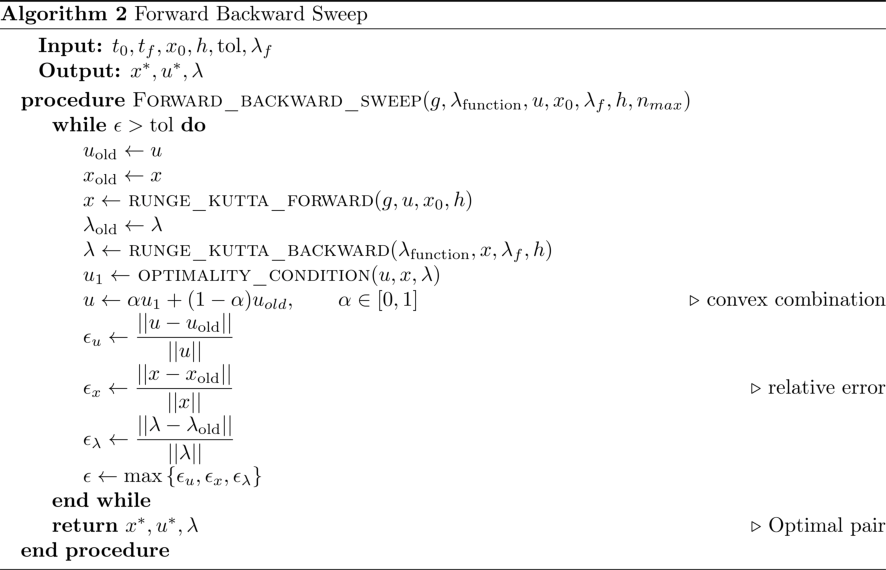
\includegraphics[width=1\linewidth]{fbs_algorithm}
\end{frame}
        \begin{frame}{SARS: isolation and quarantine}

    \begin{textblock*}{65mm}(17mm, 35mm)
     \begin{equation*}\label{eqn:sars_model}
        \begin{aligned}
            \dfrac{dS}{dt} &=
                \Lambda 
                -\dfrac{
                    S
                    \left(
                        \beta I 
                        + \mathcal{E}_E  \beta E
                        + \mathcal{E}_Q  \beta Q
                        + \mathcal{E}_J  \beta J
                    \right)
                }{N}
                - \mu S,
            \\
            \dfrac{dE}{dt} &=
                p +
                \dfrac{
                    \beta S
                    \left(
                        \beta I 
                            + \mathcal{E}_E \beta E
                            + \mathcal{E}_Q \beta Q
                            + \mathcal{E}_J \beta J
                    \right)
                }
                {N}
                -(
                    \textcolor{cyan}{u_1(t)}
                     + k_1 + \mu
                )E,
            \\
            \dfrac{dQ}{dt} &=
                 \textcolor{cyan}{u_1(t)}
                 E - (k_2 + \mu) Q,
            \\
            \dfrac{dI}{dt} &=
                k_1 E 
                -(
                    \textcolor{cyan}{u_2(t)}
                + d_1  + \sigma_1 + \mu) I,
            \\
            \dfrac{dJ}{dt} &=
                    \textcolor{cyan}{u_2(t)}
                  I 
                + k_2 Q
                - (d_2 + \sigma_2 + \mu) J,
            \\
            \dfrac{dR}{dt} &=
                \sigma_1 I
                +\sigma_2 J
                - \mu R.
        \end{aligned}
     \end{equation*}
    \end{textblock*}
        
    \begin{textblock*}{55mm}(15mm, 12mm)
            \begin{equation*}\label{eqn:sars_cost}
              \min_{u \in U}\int_{0}^{t_f}
                  \left[
                    B_1 E(t)
                    + B_2 Q(t)
                    + B_3 I(t)
                    + B_4 J(t)
                    + \frac{C_1}{2} u_1^2 (t)
                    + \frac{C_2}{2} u_2^2 (t)
                  \right]
                  dt.
            \end{equation*}
    \end{textblock*}
\end{frame}

\begin{frame}{}
    \begin{table}
        \begin{center}
            \begin{tabular}{@{}rlrl@{}}
                \toprule
                \multicolumn{4}{c}{\bf{Parameters values}}
                \\
                \midrule
                $\beta$
                & \num{0.2}
                & $d_1$, $d_2$
                & \num{0.0079}, \num{0.0337}
                \\
                $\varepsilon_E$, 
                $\varepsilon_Q$,
                $\varepsilon_J$
                & \num{0.3}, \num{0.0}, \num{0.1}
                &
                $k_1$, $k_2$ 
                & 
                \num{0.1},
                \num{0.125}
                \\
                $\mu$
                & \num{0.000034}
                \\
                $\Lambda$
                & $\mu N$
                \\
                $p$
                & \num{0.0}
                \\
                $\sigma_1$, $\sigma_2$
                & \num{0.0337}, \num{0.0386}
                && \multicolumn{1}{c}{\bf{Initial conditions}}
                \\
                \cmidrule{4-4}
                &&& $S(0)=\num{12e6}$, $E(0)=1565$,
                \\
                $t_f$
                & $\SI{1.0}{year}$
                && $Q(0)=292$, $I(0)=\num{695}$,
                \\
                Step size
                & $dt=\SI{1.0}{day}$
                && $J(0)=\num{326}$, $R(0)=\num{20}$
                \\
                $u_i$ bounds
                & \num{.05}, \num{0.5}
                \\
                $B_1$, $B_2$, $B_3$, $B_4$
                & \num{1.0}, \num{1.0}, \num{1.0}, \num{1.0}
                \\
                $C_1$, $C_2$
                & \num{300}, \num{600}
                \\
                \bottomrule
            \end{tabular}
        \end{center}
    \end{table}
\end{frame}

\begin{frame}{}
    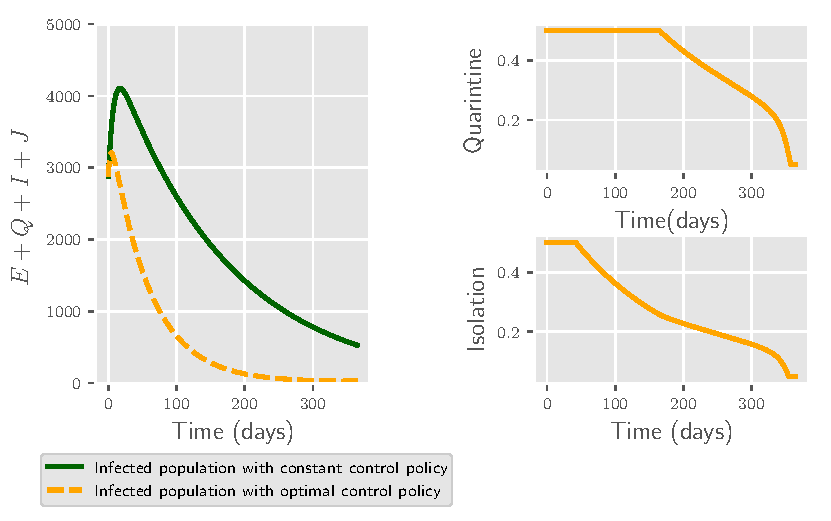
\includegraphics[width=\linewidth]{figure_1_sars-eps-converted-to.pdf}
\end{frame}
\begin{frame}{}
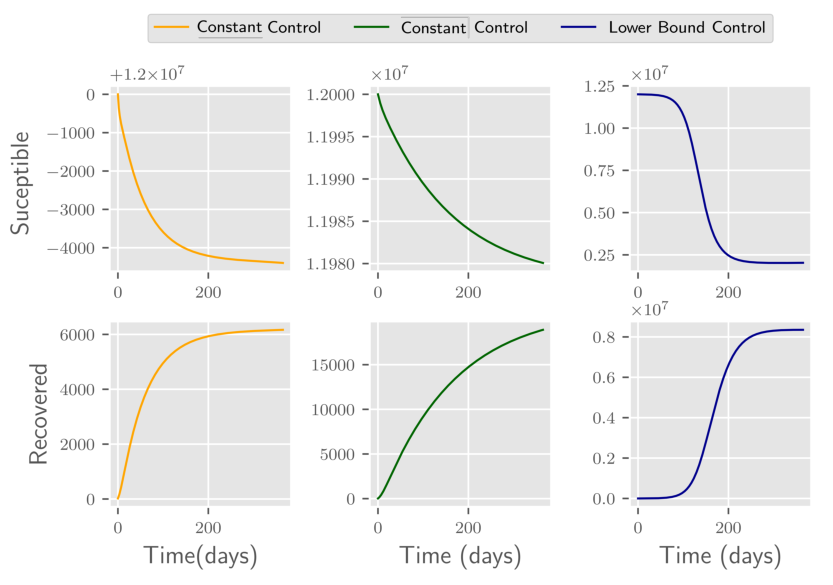
\includegraphics[width=\linewidth]{figure_2_sars-eps-converted-to.pdf}
\end{frame}
\begin{frame}{}
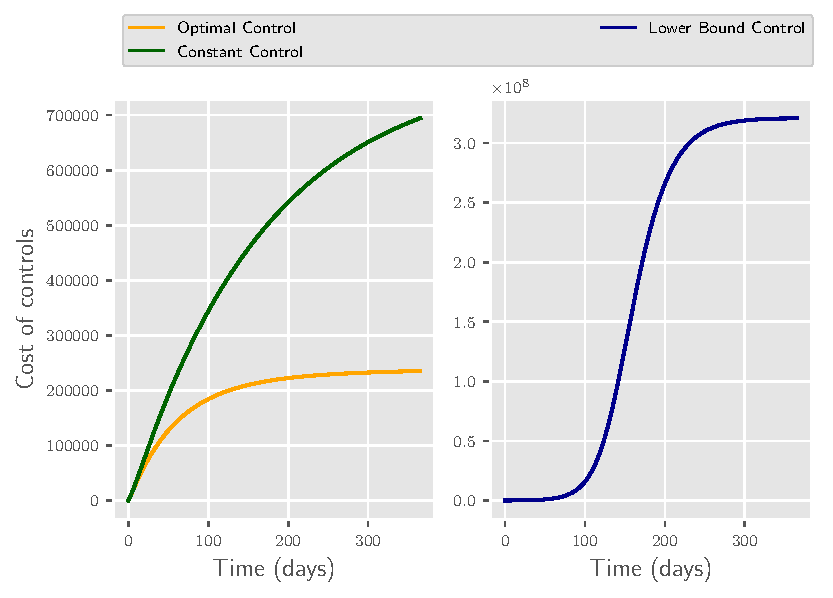
\includegraphics[width=\linewidth]{figure_3_sars-eps-converted-to.pdf}
\end{frame}
    \section{Concluding remarks}
        \begin{frame}{Concluding remarks}
    
    {\bf Uniqueness of optimal policy}.
    The proof of the uniqueness of the state path $X_u$, given a policy $u$, is
    fairly standard. However, the uniqueness of an 
    {\it optimal policy} is not trivial and it can be established on some small 
    enough interval.
    
    {\bf Numerical schemes.}
    According with the forward-backward-sweep, the 
    schemes needs a ODE solver one of its steps. However some times this solver 
    generates spurious solutions as resulting of numeric instability. 
    We see an opportunity to  apply nonstandard numerical schemes which are consistent with 
    the underlying conservation laws.
    
    Direct methods
\end{frame}
\begin{frame}{}
    
    {\bf Maximum principle vs. Dynamic programming.} 
    The same approach is followed in almost all the related literature on optimal
    control of epidemics/diseases.
    
     As an alternative, the so-called Dynamic
    programming approach can be used to analyze this kind of problems. With the
    Maximum principle we need to solve a system of ordinary differential equations
    (ODEs) whereas in Dynamic programming a partial differential equation (PDE)
    arises. In addition, both approaches involve an optimization problem. 
        
    By following the DP approach, the optimal policies are obtained in {\it feedback} (or {\it Markov}) form, i.e., the control policy is a function of the state of the system. Thus DP is a natural approach to solve stochastic models.
\end{frame}
%

        \begin{frame}{References}
            Complete list of references:
            \href{https://www.overleaf.com/read/vnvgjdqkmznc
            }{https://www.overleaf.com/read/vnvgjdqkmznc}
            
            %
            Python code:
            \nocite{python_repo}
            \bibliographystyle{amsalpha}
            \bibliography{references.bib}
        \end{frame}
\end{document}
